
受量子硬件实现中的若干物理限制影响，当前量子计算机通常被归类为含噪中等规模量子（Noisy Intermediate-Scale Quantum, NISQ）硬件。NISQ 硬件的典型特征是量子比特数量有限（约 50 到数百个）且操作含噪。此外，当前超导量子芯片的实现并不具备理想的量子比特全连接结构，而通常至多支持近邻连接。由于这些约束，大多数量子算法无法直接在 NISQ 设备上执行。为了实现算法中的双量子比特门，需要将逻辑量子比特动态重映射到物理量子比特上。这一问题称为量子比特映射问题 \cite{10323857}。

量子比特映射问题已被证明是 NP-Complete 问题 \cite{siraichi2018qubit}。考虑到时间复杂度，\MindQuantum\ 选择了一种基于 SWAP 的双向启发式算法，名为 SABRE \cite{li2019tackling}。

图 \ref{fig:qubit-mapping-sample} 给出了一个量子比特映射示例。
物理硬件有自身的物理连接图。当我们将逻辑量子比特映射到物理量子比特上时，由于两个量子比特在物理连接图中可能并不相连，某些双量子比特门可能无法直接实现。最直接的解决方案是使用 SWAP 门。通过若干 SWAP 操作，即可实现逻辑线路。

\begin{figure}
	\centering
	\begin{subfigure}{0.1\textwidth}
		\centering
		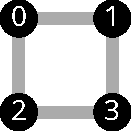
\includegraphics[width=\textwidth]{8.2_figures/example_topo}
		\caption{物理拓扑图。}
	\end{subfigure}
	\begin{subfigure}{0.3\textwidth}
		\centering
		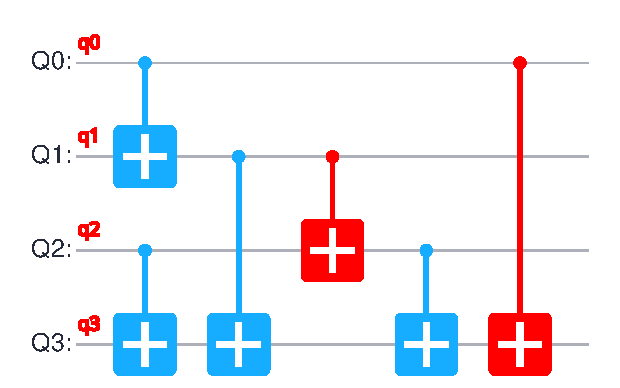
\includegraphics[width=0.9\textwidth]{8.2_figures/example_original}
		\caption{逻辑线路。}
	\end{subfigure}

	\begin{subfigure}{0.45\textwidth}
		\centering
		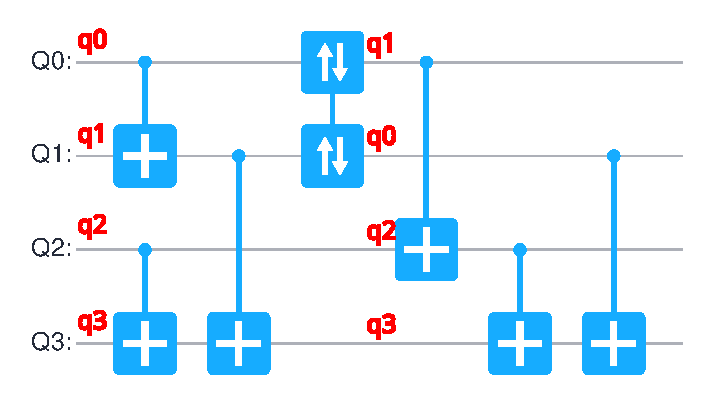
\includegraphics[width=\textwidth]{8.2_figures/example_updated}
		\caption{修正后的线路。}
	\end{subfigure}

	\caption{量子比特映射示例。}
	\label{fig:qubit-mapping-sample}
\end{figure}

该算法的目标是减少 SWAP 门数量和线路深度。

首先，可以生成一个有向无环图（DAG）来表示给定量子线路中双量子比特门之间的约束关系。单量子比特门总是可以执行，因此无需考虑。可以将每个双量子比特门标记为 $g_i(q_j, q_k)$，表示 $g_i$ 作用在 $q_j$ 和 $q_k$ 上。如果 $g_x(q_i, q_j)$ 后面跟着 $g_y(q_j, q_k)$，则向 DAG 中加入一条边 $(g_x, g_y)$。图 \ref{fig:qubit-mapping-dag} 展示了一个 DAG 生成示例。

\begin{figure}
	\centering
	\begin{subfigure}{0.49\textwidth}
		\centering
		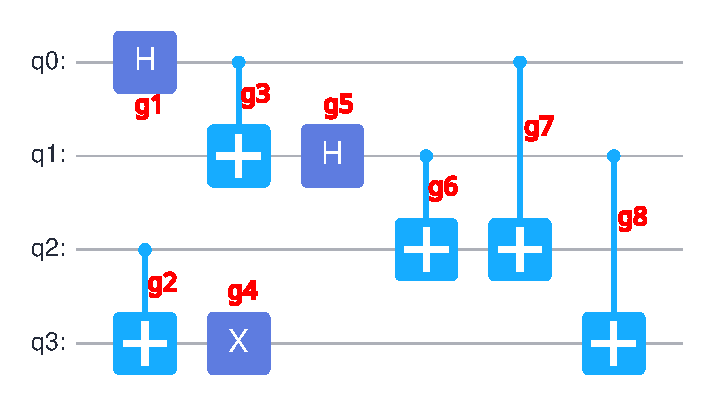
\includegraphics[width=\textwidth]{8.2_figures/dag_circuit}
		\caption{量子线路。}
	\end{subfigure}
	\begin{subfigure}{0.49\textwidth}
		\centering
		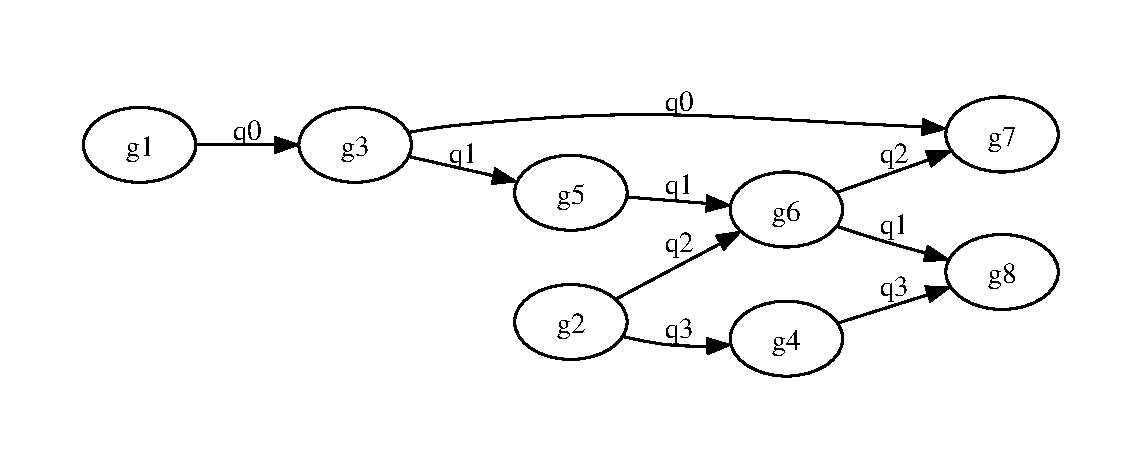
\includegraphics[width=\textwidth]{8.2_figures/dag_dag}
		\caption{生成的 DAG。}
	\end{subfigure}
	\caption{DAG 生成示例。}
	\label{fig:qubit-mapping-dag}
\end{figure}

该算法的核心思想十分直接。类似于拓扑排序，我们可以构造一个当前需要执行的前沿层。如果某个门在当前映射下可以执行，则执行该门并更新前沿层。当没有门可以执行时，计算可用的 SWAP。最后，选择启发式函数值最小的 SWAP。

基础启发式函数来自最近邻代价函数。对于两个物理量子比特 $Q_i$ 和 $Q_j$，$D[Q_i][Q_j]$ 表示二者在物理连接图中的最短距离。对于给定前沿层 $F$ 和当前映射 $\pi$，基础函数定义见式 \eqref{eq:qubit-mapping-h-basic}。
\begin{equation} \label{eq:qubit-mapping-h-basic}
	H_{\text{basic}} = \sum_{g \in F} D[\pi (g.q_1)][\pi (g.q_2)].
\end{equation}

$H_{\text{basic}}$ 只考虑前沿层。如果希望进行前瞻，可以加入一个扩展集合 $E$，其中包含来自 $F$ 的若干最近后继门。$E$ 的大小是灵活的，取决于所需的前瞻能力。同时，$F$ 中的门应具有比 $E$ 更高的优先级。因此，引入权重参数 $0 \leq W < 1$。

到目前为止，该启发式函数倾向于减少 SWAP 门数量。我们还希望降低线路深度，二者之间存在权衡。为此，为每个量子比特加入一个 $decay$ 参数。如果某个量子比特上已经执行了很多操作，则它会具有更大的 $decay$。借助 $decay$，算法会倾向于选择操作较少的量子比特，从而提高线路并行度。修正后的启发式函数见式 \eqref{eq:qubit-mapping-h}。
\begin{equation} \label{eq:qubit-mapping-h}
	\begin{aligned}
		H =    & \max \left( \rm{decay}(\rm{SWAP.q_1}), \rm{decay}(\rm{SWAP.q_2}) \right)                \\
		\times & \Big\lbrace \frac{1}{|F|} \sum_{g \in F} D[\pi(g.q_1)][\pi(g.q_2)]  \\
		+      & \frac{W}{|E|} \sum_{g \in E} D[\pi(g.q_1)][\pi(g.q_2)] \Big\rbrace.
	\end{aligned}
\end{equation}

最后，还需要处理初始映射问题。已有研究表明，初始映射会对最终结果产生巨大影响。这里我们采用文献 \cite{li2019tackling} 中介绍的方法。图 \ref{fig:qubit-mapping-initial-mapping} 展示了更新初始映射的过程。

\begin{figure}
	\centering
	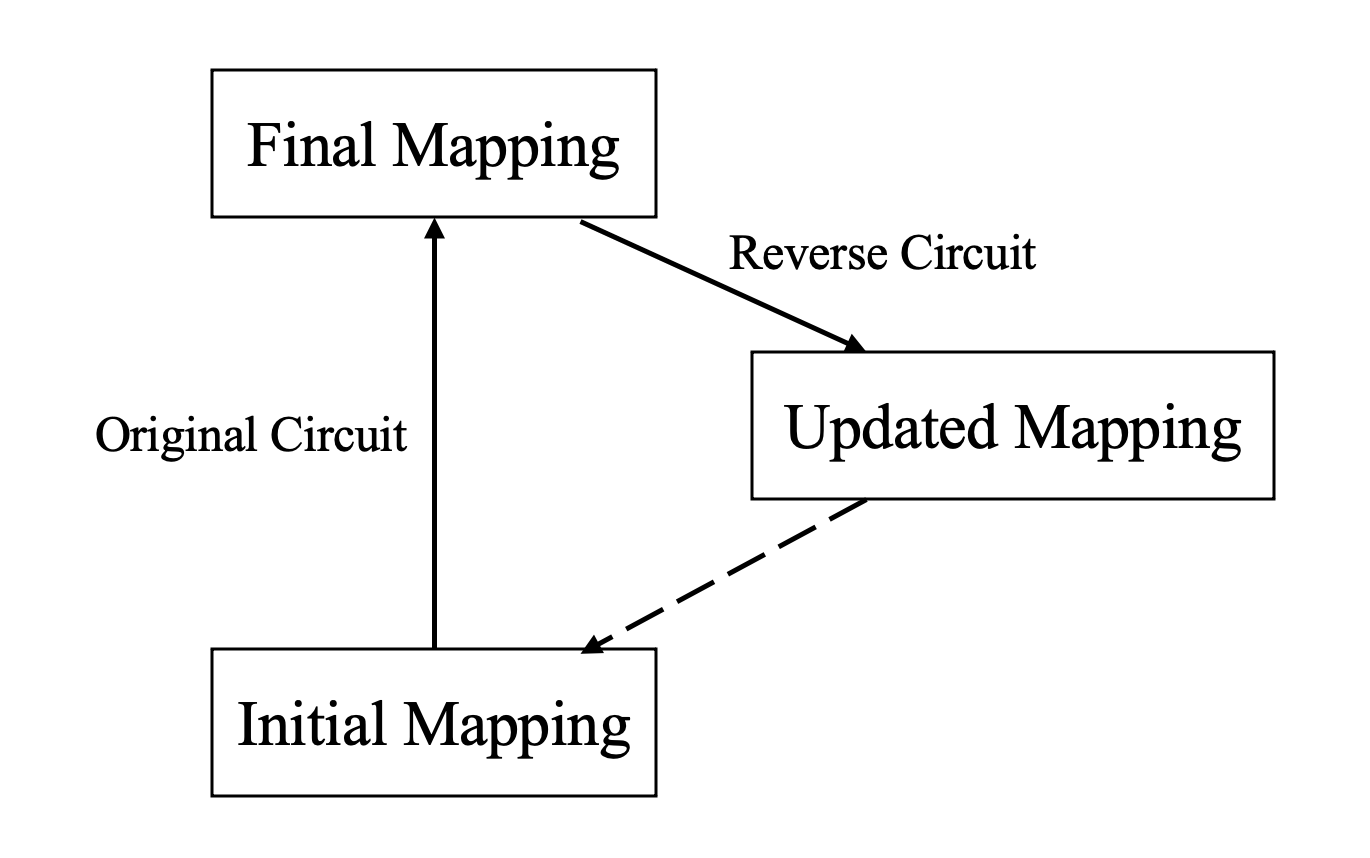
\includegraphics[width=0.45\textwidth]{8.2_figures/initial_mapping.png}
	\caption{初始映射更新过程。}
	\label{fig:qubit-mapping-initial-mapping}
\end{figure}

下面介绍如何在 \MindQuantum\ 中使用 SABRE。可以使用 \code{QubitNode} 和 \code{QubitsTopology} 生成物理拓扑图。

\begin{lstlisting}
from mindquantum.device import QubitNode, QubitsTopology
from mindquantum.io.display import draw_topology

n: int = 5
topology = QubitsTopology([QubitNode(i, poi_x=i) for i in range(n)])
draw_topology(topology)
\end{lstlisting}

上述代码定义了一个包含 5 个节点的拓扑图。\code{QubitNode(i, poi_x=i)} 定义了一个 ID 为 \code{i}、x 轴坐标为 \code{i} 的 \code{QubitNode}。\code{draw_topology} 用于绘制图 \ref{fig:qubit-mapping-topo1} 所示的 SVG。

\begin{figure}
	\centering
	\begin{subfigure}{0.2\textwidth}
		\centering
		
\includegraphics[width=0.8\textwidth]{8.2_figures/topo_1}
		\caption{非连通图。}
		\label{fig:qubit-mapping-topo1}
	\end{subfigure}
	\begin{subfigure}{0.2\textwidth}
		\centering
		
\includegraphics[width=0.8\textwidth]{8.2_figures/topo_2}
		\caption{连通图。}
		\label{fig:qubit-mapping-topo2}
	\end{subfigure}
	\caption{定义一个包含 5 个节点的拓扑图。}
\end{figure}

也可以使用 \code{q1 >> q2} 或 \code{q1 << q2} 连接不同节点，并使用 \code{q1 > q2} 或 \code{q1 < q2} 断开节点连接。下面的代码连接图 \ref{fig:qubit-mapping-topo1}，并生成图 \ref{fig:qubit-mapping-topo2}。

\begin{lstlisting}
for i in range(n-1):
    topology[i] << topology[i+1]
draw_topology(topology)
\end{lstlisting}

\MindQuantum\ 还定义了一些有用的结构。下面的代码定义了图 \ref{fig:qubit-mapping-linear} 所示的线性拓扑，以及图 \ref{fig:qubit-mapping-grid1} 所示的网格拓扑。

\begin{lstlisting}
from mindquantum.device import LinearQubits, GridQubits

t1 = LinearQubits(3)
t2 = GridQubits(3,4)
draw_topology(t1)
draw_topology(t2)
\end{lstlisting}

也可以修改已有图。下面的代码会删除一个节点、孤立一个节点、改变一个节点的颜色、改变一个节点的位置，并添加一条新边。图 \ref{fig:qubit-mapping-grid2} 展示了修改后的图。

\begin{figure}[H]
	\centering

	\begin{subfigure}{0.1\textwidth}
		
\includegraphics[width=0.9\textwidth]{8.2_figures/linear}
		\caption{线性拓扑。}
		\label{fig:qubit-mapping-linear}
	\end{subfigure}
	\begin{subfigure}{0.15\textwidth}
		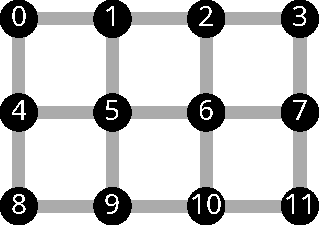
\includegraphics[width=0.9\textwidth]{8.2_figures/grid1}
		\caption{网格拓扑。}
		\label{fig:qubit-mapping-grid1}
	\end{subfigure}
	\begin{subfigure}{0.2\textwidth}
		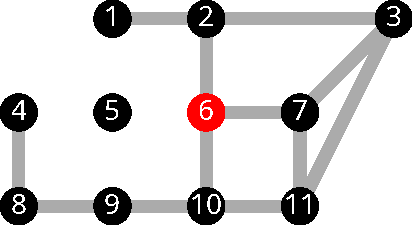
\includegraphics[width=0.9\textwidth]{8.2_figures/grid2}
		\caption{修改后拓扑。}
		\label{fig:qubit-mapping-grid2}
	\end{subfigure}

	\caption{若干常用结构与修改后的拓扑图。}
\end{figure}

\begin{lstlisting}
t2.remove_qubit_node(0)
t2.isolate_with_near(5)
t2.set_color(6, "#ff0000")
t2.set_position(3, 4, 0)
t2[3] << t2[11]
draw_topology(t2)
\end{lstlisting}

结合给定拓扑图，可以使用 SABRE 算法为任意逻辑量子线路生成量子比特映射。下面的代码定义了一个拓扑图 \code{topo} 和一个逻辑线路 \code{circ}。SABRE 求解器需要 4 个参数：
\begin{itemize}
	\item \code{iter_num}：生成初始映射的迭代次数。
	\item \code{w}：式 \eqref{eq:qubit-mapping-h} 中的 $W$ 参数。
	\item \code{delta1}：单量子比特门的衰减参数。
	\item \code{delta2}：CNOT 门的衰减参数。
\end{itemize}
求解器返回三部分：
\begin{itemize}
	\item \code{new_circ}：物理线路。
	\item \code{initial_mapping}：表示初始映射的列表。这里，小写 $q$ 表示逻辑量子比特，大写 $Q$ 表示物理量子比特。例如，\code{[3, 2, 0, 1]} 表示逻辑 $q_0$ 存储在物理 $Q_3$ 上，$q_1$ 存储在 $Q_2$ 上，$q_2$ 存储在 $Q_0$ 上，$q_3$ 存储在 $Q_1$ 上。
	\item \code{final_mapping}：表示最终映射的列表。
\end{itemize}
图 \ref{fig:qubit-mapping-physical-circuit} 展示了一种可能的解。

\begin{lstlisting}
topo = GridQubits(2, 2)
display_svg(draw_topology(topo))

from mindquantum.core.circuit import Circuit
from mindquantum.algorithm.mapping import SABRE

circ = Circuit().h(0).h(1).h(2).x(1, 0).x(2, 1).x(0, 2)
print("Logical circuit:")
display_svg(circ.svg())

solver = SABRE(circ, topo)
new_circ, init_mapping, final_mapping = solver.solve(5, 0.5, 0.3, 0.2)
print("Physical circuit:")
print(f"initial mapping: {init_mapping}")
print(f"  final mapping: {final_mapping}")
display_svg(new_circ.svg())
\end{lstlisting}

\begin{figure}
	\centering
	\begin{subfigure}{0.1\textwidth}
		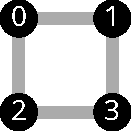
\includegraphics[width=0.8\textwidth]{8.2_figures/topo_3}
		\caption{物理拓扑图。}
		\label{fig:qubit-mapping-physical-topo}
	\end{subfigure}
	\begin{subfigure}{0.35\textwidth}
		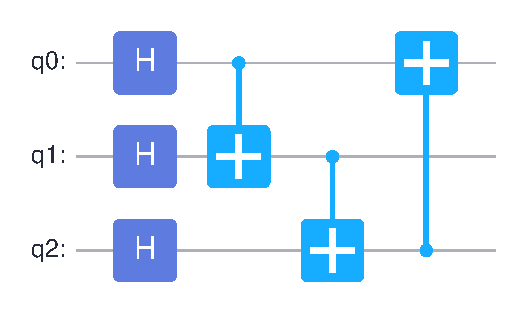
\includegraphics[width=\textwidth]{8.2_figures/logical}
		\caption{逻辑线路。}
		\label{fig:qubit-mapping-logical-circuit}
	\end{subfigure}
	\begin{subfigure}{0.45\textwidth}
		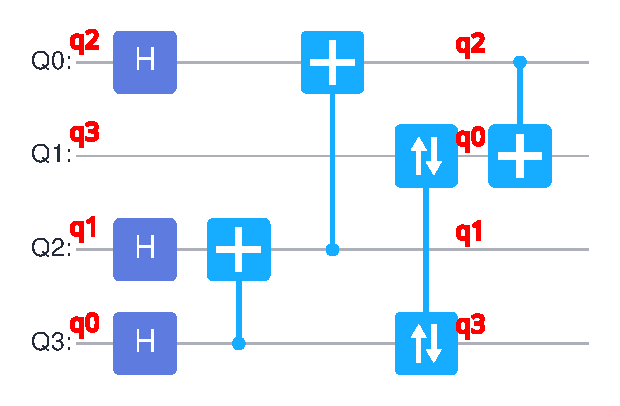
\includegraphics[width=0.9\textwidth]{8.2_figures/physical}
		\caption{一种可能的物理线路。初始映射为 \code{[3, 2, 0, 1]}，最终映射为 \code{[1, 2, 0, 3]}。}
		\label{fig:qubit-mapping-physical-circuit}
	\end{subfigure}

	\caption{SABRE 算法示例。}
\end{figure}

该实现也存在一些不足。目前 \MindQuantum\ 仅支持连通拓扑图。如果物理拓扑不连通，用户必须手动将逻辑量子比特分配到物理连通子图中。
另一个限制是门类型。当前版本只支持单量子比特门和 CNOT 门。由于任意量子线路都可以由单量子比特门和 CNOT 门实现，因此这并不是严重问题。

% Test \code{hello world} .
% - Eq.~\eqref{}
% - Fig.~\ref{}
% - \code{}
